\documentclass[a4paper,10pt]{report} % {article}
% ==== Header for document with math =========

% --- input -----------------------------------
  \usepackage[utf8]{inputenc}
  \usepackage[base]{babel}  
  
% --- math -----------------------------------
  \usepackage{amsmath}
  \usepackage{amsfonts}
  \usepackage{amstext}
  \usepackage{amssymb}
  \usepackage{amsthm}
  

% --- graphic and formating ------------------
  % bibliography
  \usepackage[sort,comma]{natbib}
  % settings
  \usepackage{enumitem}
  \usepackage{setspace}
  \usepackage{pdflscape}
  \usepackage{graphicx}
  \usepackage{wrapfig}
  \usepackage[hypcap]{caption}
  \usepackage{subcaption}
  % \usepackage[cm]{fullpage}
  \usepackage[top=2cm, bottom=1.7cm, left=3.6cm, right=1.1cm]{geometry}
  % \usepackage[leftmargin=2.5cm]{geometry}
  %\usepackage{subfigure}
  %\usepackage{caption}
  %\usepackage{subcaption}  
  \usepackage{placeins}
  \usepackage{makeidx} 
  \usepackage{epstopdf}
  % \usepackage{tocloft}     % custom lists
  % \usepackage{minitoc}     % table of content in a chapter
  
   \usepackage{listings}     % code listings
  % \usepackage[printwatermark]{xwatermark} % \usepackage{draftwatermark}
  
  \usepackage[colorlinks=true,linkcolor=interlink,citecolor=DarkCite]{hyperref}
  
  % \usepackage{picture}
  \usepackage[usenames,dvipsnames]{color}
  \usepackage{colortbl} 
  

   \setlength{\headsep}{16pt}
%    
   \usepackage{fancyhdr}
   % ---- fancy page setting -------------- 
   %\input{./latex/style_header_footer.tex}
   \fancyhead[l]{\color{gray}{19. and 21. June 2023}}
\fancyhead[r]{\color{gray}{Informal LaTeX workshop}} % {Exam METABL ~---~ August 1, 2018}
\fancyfoot[l]{\color{gray}{intermediate and advanced topics}}
\fancyfoot[c]{\color{gray}{- \thepage/\pageref*{LastPage} -}}
\fancyfoot[r]{\color{gray}{\( \star \)}} 
\setlength{\headheight}{18pt}
    \renewcommand{\headrulewidth}{1pt}
    \renewcommand{\footrulewidth}{1pt}

   %----------------------------------------
  
  % picture libraries
  \usepackage{tikz} % Required for flow chart
   \usetikzlibrary{arrows,positioning} % Tikz libraries required for the flow chart in the template
   
       \tikzset{
        %Define standard arrow tip
        >=stealth',
        %Define style for boxes
        point/.style={
           rectangle,
           rounded corners,
           draw=black, very thick,
           text width=6.5em,
           minimum height=2em,
           text centered},
        % Define arrow style
        pil/.style={
           ->,
           thick,
           shorten <=2pt,
           shorten >=2pt,}
    }

   \usepackage{csvsimple}  % csv table
   
   \usepackage{lipsum}    % filler text
   
   
  %\hypersetup{
    % bookmarks=false,         % show bookmarks bar?https://www.overleaf.com/project/637266f5927ea984e19f515e
    % unicode=false,          % non-Latin characters in Acrobat’s bookmarks
    % pdftoolbar=false,        % show Acrobat’s toolbar?
    % pdfmenubar=false,        % show Acrobat’s menu?
%     % pdffitwindow=false,     % window fit to page when opened
    % pdfstartview={FitH},    % fits the width of the page to the window 
    %pdfauthor={Author},     % author
    %pdfsubject={Subject},   % subject of the document
    %pdfcreator={Creator},   % creator of the document
    %pdfproducer={Producer}, % producer of the document
    %pdfkeywords={keyword1, key2, key3}, % list of keywords
    % pdfnewwindow=true,      % links in new PDF window
  \hypersetup{
    pdfinfo={
        Title={Informal LaTeX workshop},
        Author={InScAPE group},
        Creator={Your Name Here},
        Producer={Institute for Geophysics and Meteorology},
        Subject={Informal LaTeX workshop on intermediate and advanced topics},
        Keywords={tables, tikz, counters}
    },
    colorlinks=true,            % false: boxed links; true: colored links
    linkcolor= ref_out,         % color of internal links
    linkbordercolor = red,      % color of box around links 
    citecolor=green,            % color of links to bibliography
    filecolor=cyan,             % color of file links
    urlcolor=magenta,           % color of external links
    urlbordercolor = {0 0.6 1}  % (change box color with linkbordercolor)
    % pdfborderstyle={/S/U/W 1} % border style will be underline of width 1pt
} 

% ---- new commands --------------------------
  % ----- link colours ------------
    \newcommand{\reffig}[1]%
    {\hypersetup{linkcolor=figlink}%
    \ref{#1}%
    \hypersetup{linkcolor=interlink}}
 
  % ---- math symbols  ----------------------- 
  \newcommand{\e}{\mathrm{e}}
  \newcommand{\dx}{\mathrm{d}}
  \newcommand{\normal}{\mathbi{n}}
  \newcommand{\bsigma}{\mathbf{t}}
  \newcommand{\vnull}{\mathbf{0} \!\!\! ^{ _{ _{\scriptscriptstyle -}}}}
  \newcommand{\vnullt}{\mathbf{0}^{ \mathrm{T} \!\!\!\!\!\!\! \! _{ _{\scriptscriptstyle -}}}}
  % ---- math fonts -------------------------- 
  \newcommand{\mathbs}[1]{\textsf{#1}}
  \newcommand{\mathbi}[1]{\textbf{\emph #1}}
  \newcommand{\mathff}{\textbf{\textit f}}
  \newcommand{\mathbis}[1]{\textsf{\em #1}}
  \newcommand{\mathcb}[1]{\boldsymbol{\mathcal #1}}
  
  
\newcommand{\thv}{\theta_{\scriptscriptstyle \mathcal{V} }}
\newcommand{\thml}{\theta^{\scriptscriptstyle \mathrm{(ML)}}}

  % --- modifying existing commands -------------------
  

  
  % ---- our own Macros  --------------------------
  
  %  our own lists 
%  \newcommand{\listoflists}{List of Lists}  % we add a list
  
%  \newlistof{lists}{tol}{\listoflists}      % list itself 
  
%  \newcommand{\list}[1]{%
%    \refstepcounter{lists}
%    \par\noindent\textbf{lists \theexample. #1}
%    \addcontentsline{tol}{list}
%    {\protect\numberline{\thechapter.\theexample}#1}\par
  
  

% ---- latex commands -----------------------
  % --- graphic commands --------------------
  \DeclareGraphicsExtensions{.png,.jpg}

  % --- colour definition ------------------
  % colour definition
  \definecolor{GreenDone}{rgb}{0.2,0.7,0.2}
  \definecolor{lightorange}{rgb}{0.9,0.4,0}
  \definecolor{lightestorange}{rgb}{1,0.8,0.5}
  \definecolor{darkorange}{rgb}{0.2,0.1,0}
  \definecolor{interlink}{rgb}{0.6,0,0}
  \definecolor{DarkCite}{rgb}{0,0.3,0}
  % \definecolor{ref_out}{rgb}{0.3,0.3,0}
  \definecolor{ref_out}{rgb}{0.6,0,0}
  \definecolor{lightyellow}{rgb}{0.99,0.99,0.4}
  \definecolor{UeaBlue}{RGB}{0,76,103}
  \definecolor{LightBlue}{RGB}{20,20,250}
  \definecolor{DarkBlue}{RGB}{15,10,100}  
  \definecolor{figlink}{RGB}{45,10,120} 
  \definecolor{bordercol}{RGB}{40,40,40}
  \definecolor{headercol1}{RGB}{186,215,230}
  \definecolor{headercol2}{RGB}{0,76,103}
  \definecolor{headerfontcol}{RGB}{0,0,0}
  \definecolor{boxcolor}{RGB}{186,215,230}


\title{Advanced LaTeX Workshop}
\author{Your Name Here}
\date{19 June 2023} 

\pdfinfo{%
  /Title    (Advance LaTeX Workshop) 
  /Author   (Your Name Here)
  /Creator  (Your Name Here)
  /Producer (InScAPE)
  /Subject  (Intermediate and Advanced LaTeX)
  /Keywords (listing, tikz, figures) 
}
 
\begin{document}
% later: #4 generating index 
%--------------
%\makeindex
%--------------

\maketitle

% \maketitle
 \pagestyle{fancy}
 %\setcounter{page}{1}
 \pagenumbering{roman}

 \section*{Introduction} 
 
 This document is a guidebook on intermediate and advanced topics in \LaTeX, with a target audience of researchers and other professionals who often have to use \LaTeX.\\
 
 
 This guidebook was originally started for the purpose of a informal workshop held at the University of Cologne. 
 The original overview follows:
 \\~\vspace{5ex}
 
%-------- Workshop overview-------------------------------
\begin{tabular}{|p{0.8\textwidth}}
 \textcolor{gray}{
 We are organising an informal \textbf{workshop} on the \textbf{intermediate and advanced topics} in \LaTeX.
Although there are various \LaTeX tutorials and templates floating around, but they often omit some tools and packages that are useful in meteorology and geophysics. The workshop is primary focused on PhD students who are starting to write their thesis, but it is open to other \LaTeX users as well.}
\\
 \begin{enumerate}
 \item   \textcolor{gray}{Monday 19. June --- from 12:45 in CIP room}
 \item   \textcolor{gray}{Wednesday 21. June --- from 15:00 in CIP room} 
\end{enumerate}\\


\noindent
 \textcolor{gray}{ You can work from CIP workstation or bring your own device.}~\vspace{3ex}\\
\end{tabular}
 

 \begin{tabular}{l p{0.7\textwidth}}
   \textcolor{gray}{target audience:} & \textcolor{gray}{people with previous experience with \LaTeX} \\
   \textcolor{gray}{aims:}  & \textcolor{gray}{discuss \LaTeX ~topics practise skills} \\
   \textcolor{gray}{duration:} & \textcolor{gray}{one and half hour from start time or until you start getting tired} \\
   \textcolor{gray}{topics:} & \textcolor{gray}{see following sections \ref{sec:monday} and \ref{sec:wednesday}} \\
   \textcolor{gray}{registration:} & \textcolor{gray}{comment in this Slack thread} \\ 
 \end{tabular}
 
 \pagebreak


%-----------------------------------------------------------------------------
 
\section{Monday} \label{sec:monday}




\subsection{Combining Document from Pieces}
Combining documents from multiple files speeds up the editing process, makes collaboration easier, and also lowers the risk of accidentally rewriting something. You can see an example how most of the header of this document is in a separate file.\\

\lstinputlisting[ language={[latex]tex},      % tex syntax, latex option
  caption={Input statement}, label={code:input}, 
  firstline=1, firstnumber=1, lastline=3, numbers=left, captionpos=b,
  frame=single,
  basicstyle=\footnotesize\color{darkgray}, 
  keywordstyle=\bf\color{magenta},
  commentstyle=\color{ForestGreen},  %
  breaklines=true
]{./day1latex_adjusted1.tex} 

The input statements could be then again used in the file that was itself inputted:

\lstinputlisting[ language={[latex]tex},      % tex syntax, latex option
  caption={Input statement inside in1header.tex}, label={code:input2}, 
  firstline=50, firstnumber=50, lastline=54, numbers=left, captionpos=b,
  frame=single, 
  basicstyle=\footnotesize\color{cyan},
  keywordstyle=\color{magenta}, stringstyle=\color{brown}, commentstyle=\color{gray},
  breaklines=true
]{./latex/in1header.tex} 

% #1 
To try this, write some dummy text in a separate file and insert is here using the \texttt{input} command:\\
\input{./data/just2lines.txt}\\


% #2 
The \texttt{input} statement can also work on multiple levels
\begin{enumerate}
    \item Make a copy of \texttt{style1headerfooter.tex} and modify it.
    \item Open \texttt{in1header.tex} and replace \texttt{style1headerfooter.tex} with the name of your new file.
    \item Recompile the main document.
\end{enumerate} 



\subsection{Automatically Generated Lists} %\label{sec:automatic}
There is an easy way how to create list of figures, tables, as well as index of phrases. 
 See on the following page: 

% We are going to start witth this documet
%  #1 change the class of document from article to report
%  



%\pagenumbering{roman}
%   \let\clearpage\relax 
   \tableofcontents
    \label{contents}
   \addcontentsline{toc}{section}{Table of Contents}  
   \let\clearpage\relax
   \addcontentsline{toc}{section}{List of Tables}
    \listoftables  
  \let\clearpage\relax
   \addcontentsline{toc}{section}{List of Figures}  
   \listoffigures\label{lof}  
    \chapter*{List of Symbols}
   \addcontentsline{toc}{section}{List of Symbols}
   % ========================
% list  of symbols
%=======================
\begin{onehalfspace}
\begin{tabular}{l l p{0.7\textwidth} }
\hline
		notation  & unit & meaning \\
\hline \\
		\( \sim \) & \( \cdot \) & similar - assignment of probability distribution\\	
		\( \propto \) & \( \cdot \) & proportional equivalent to; i.e.  equivalent up to a constant\\
		\( \overline{(\; \cdot \;)} \) & \( \cdot \) & horizontal averaging \\
		\( \overline{\varphi} \) & 	\( \cdot  \) & mean value of a quantity \( \varphi \)  \\
% 		\( \overline{\varphi}^{(l,k)} \) & 	\( \cdot  \) & mean value of a quantity \( \varphi \) over a subdomain \\		
% 		\( \varphi^{\prime}\) & 	\( \cdot  \) & variant part of a quantity \( \varphi \)  \\			
% 		\( \overline{(\; \cdot \;)}_{u}^{(u)} \) & \( \cdot \) &  averaging over the area of strong updraughts \\
% 		\( {(\; \cdot \;)}_{RE}\) & \(\ \cdot \) &  resolved values of a term in parenthesis\\
% 		\( \overline{(\; \cdot \;)}_{SG}\) & \(\ \cdot \) &  statistics of modelled subgrid values of a term in parenthesis\\	
% 		\( {(\; \varphi \;)}_{(\mathrm{sm}),\lambda}  \) & \( \cdot \) & smoothing of a series of variable \( \varphi \)  over smoothing length \(\lambda \) \\	
% 		
% 		\( \triangle_{\varphi}\) & \( \cdot \)  & perturbation in a quantity \( \varphi \) \\
% 		\\
% 		
% 		\( a_u \) & \( \mathrm{m} \mathrm{s}^{-1}  \) & fraction of the area taken by strong updraughts \\	
% 		
% 		\( C_{p} \)  & \(\mathrm{J} \; \mathrm{kg}^{-1} \, \mathrm{K}^{-1}  \) & specific heat capacity at constant pressure (isobaric mass heat capacity)\\
% 		
% 		\( d_{\mathrm{(h)}} \) & \( \mathrm{m} \) & length of a side of block in a heterogeneity pattern \\			
% 		\( E_{k} \)  & \(\mathrm{J} \; \mathrm{kg}^{-1}  \) & kinetic energy per unit of mass\\
% 		\( E_{w} \)  & \(\mathrm{J} \; \mathrm{kg}^{-1}  \) & kinetic energy of vertical motion\\
% 		\( h^{(\varphi)}_i  \) & \( \cdot \) & scalar flux of the quantity \( \varphi \) \\
% 		\( L_{e} \)  & \(\mathrm{J} \; \mathrm{kg}^{-1} \) & latent heat of evaporation \\
% 		
% 		
% 		\( N \)  & \( \scriptstyle{1} \) & number of gridpoints / number of measurements in a timeseries  \\
% 		\( N_{x} \)  & \( \scriptstyle{1} \) & number of gridpoints in the direction of the axis-\(x\)\\
% 		\( \mathsf{N}(\mu,\sigma^{2}) \)  & \( \cdot \) & normal distribution with mean \( \mu \) and standard deviation \(\sigma \)  \\
% 
% 		\( r \)  & \( \mathrm{kg} \; \mathrm{kg}^{-1} \) & water vapour mixing ratio \\	
% 		%-> do we use this one ?
% 		\( r_{l} \)  & \( \mathrm{kg} \; \mathrm{kg}^{-1} \)  & liquid water mixing ratio\\
% 		\( r_{\varphi} \)  & \( \cdot \)  & residua in a series of the variable \( \varphi \) \\
% 		
% 		\( q_{v} \)  & \( \mathrm{kg} \; \mathrm{kg}^{-1} \) & specific humidity \\
% 		\( q_{cl} \)  & \( \mathrm{kg} \; \mathrm{kg}^{-1}  \)  & cloud total water content \\
% 		\( q_{i} \)  & \( \mathrm{kg} \; \mathrm{kg}^{-1}  \)  & cloud ice water content \\
% 		\( q_{l} \)  & \( \mathrm{kg} \; \mathrm{kg}^{-1}  \)  & cloud liquid water content \\
% 		\( q_{t} \)  & \( \mathrm{kg} \; \mathrm{kg}^{-1}  \)  & total water content (total humidity) \\
% 
% 		\( q_{tr} \)  & \( \; \mathrm{kg}^{-1}  \)  & content of a passive aerosol tracer\\	
% 		
% 		\( Q_{LH} \)  & \( \mathrm{W} \, \mathrm{m}^{-2} \) & latent heat flux \\
% 		\( Q_{SH} \)  & \( \mathrm{W} \, \mathrm{m}^{-2} \)  & sensible heat flux \\
% 		
% 		\( P( A ) \)  & \( \cdot \)  & probability of an event A \\
% 		
% 		\\ \hline
	\end{tabular}
    \end{onehalfspace}

%   \begin{onehalfspace}
%   \begin{tabular}{l l p{0.7\textwidth} }
%   \hline
% 		notation  & unit & meaning \\
% 		\hline \\
% 		\( \mathbb{S}_{i,j} \) & \( \mathrm{s}^{-1} \) & rate of strain tensor \\
% 		\( S \) & \( \mathrm{s}^{-1} \) & modulos of the rate of strain tensor \\
% 		\( S_{\varphi,\alpha} \) & \( \cdot \) &  sample quantile of values of variable \( \varphi \) for probability \(alpha \)\\
% 		
% 		\( t_0 \)  & \( \mathrm{s} \)  & time of transition - when the surface starts warming\\	
% 		\( T \)  & \( \mathrm{K} \)  & absolute temperature\\		
% 		
% 		\( \mathbi{u} \) & \( \mathrm{m} \mathrm{s}^{-1}  \) &  vector of wind velocity  \\
% 		
% 		\( u \) & \( \mathrm{m} \mathrm{s}^{-1}  \) &  component of wind velocity in the direction of axis-\(x\)  \\
% 		
% 		\( \mathsf{U}(a,b) \)  & \( \cdot \) & uniform distribution on the interval \([a,b] \) \\
% 		\( v \) & \( \mathrm{m} \mathrm{s}^{-1}  \) &   component of wind velocity in the direction of axis-\(y\)  \\
% 		\( v_f \) & \( \mathrm{m} \mathrm{s}^{-1}  \) & large scale wind forcing in the direction of  axis-\(y\) \\		
% 		\( w \) & \( \mathrm{m} \mathrm{s}^{-1}  \) &  vertical component of wind velocity \\
% 		
% 		\( w_u \) & \( \mathrm{m} \mathrm{s}^{-1}   \) & vertical velocity in strong updraughts\\
% 		\( \overline{(w^{\prime} \varphi^{\prime})} \) & 	\( \cdot \) & vertical flux of scalar quantity; general notation \\
% 		\( \overline{(w^{\prime} \varphi^{\prime})}_{s} \) & 	\( \cdot \) & vertical flux of scalar quantity at the surface; general notation \\			
% 
% 		\( \overline{(w^{\prime} \theta^{\prime})} \) & 	\( \cdot \) 	& vertical kinematic heat flux \\ % ? adjust name? 
% 		\( \overline{(w^{\prime} \theta^{\prime}_{v})} \) & 	\( \cdot \) 	& vertical kinematic buoyancy flux \\ % ? adjust name? 
% 		\( \overline{(w^{\prime} q^{\prime})} \) & 	\( \cdot \) 		& vertical kinematic moisture flux\\ % ? adjust name ?	
% 		
% 		\( z_{0,\mathrm(vec)} \) 	& \( \mathrm{m}  \) & aerodynamic roughness length\\
% 		\( z_{0,\mathrm(vec)} \) 	& \( \mathrm{m}  \) & aerodynamic roughness length for wind \\
% 		\( z_{0,\theta} \) 		& \( \mathrm{m}  \) & aerodynamic roughness length for scalar quantities\\
% 		\( z_i \) & \( \mathrm{m}  \) & height of the mixed boundary layer (MBL) \\	
% 		\( \mathsf{z}_{\alpha} \) & \scriptsize{1}  &   quantile of the standard normal distribution for probability \(\alpha\)\\
% 		
% 		\( \delta_{i,j} \) &  \scriptsize{1} & Kronecker delta\\
% 		
% 		%-> change this one?
% 		\( \delta_{\mathrm{(h)}} T \) & \( \mathrm{K} \) & temperature scale of a heterogeneity in surface potential temperature\\
% 		\( \delta t \) & \( \mathrm{s} \) & length of timestep in a timeseries \\
% 		\( \Delta t \) & \( \mathrm{s} \) & length of a  timestep of numerical computations \\
% 		\( \Delta x \) & \( \mathrm{m} \) & grid resolution in the direction of x-axis \\
% 		\( \Delta z \) & \( \mathrm{m} \) & grid resolution in the vertical direction \\		
% 		\( \Delta_{\mathrm{(h)}} T \) & \( \mathrm{K} \) & temperature scale of a surface anomaly \\
% 		%-> check this one		
% 		\( \varepsilon_{i,j,k} \) &  \scriptsize{1} & Levi-Civita symbol in three dimensions\\
% 		\( \theta \)  & \( \mathrm{K} \)  & potential temperature \\
% 		\( \theta_{e} \)  & \( \mathrm{K} \)  & equivalent potential temperature \\		
% 		% \( \theta_{v} \)  & \( \mathrm{K} \)  & virtual potential temperature \\
% 		% \( \theta \)  & \( \mathrm{K} \)  & potential temperature \\
% 		\( \theta_{\mathrm{surf}} \) & \( \mathrm{K} \) & surface potential temperature\\	
% 		\( \theta_{v} \)  & \( \mathrm{K} \)  & virtual potential temperature \\
% 	      \\ \hline
% 	\end{tabular}
%       \end{onehalfspace}

%       \begin{onehalfspace}
%       \begin{tabular}{l l p{0.7\textwidth} }
% 	    \hline
% 	    	notation  & unit & meaning \\
% 	    \hline \\
% 		\( \kappa \) & \scriptsize{1} & Von Kármán constant \\
% 
% 
% 		\( \lambda \) & \( \mathrm{m} \) & mixing length \\
% 		\( \lambda_0 \) & \( \mathrm{m} \) & reference mixing length \\		
% 		\( \nu_m \) & \( \mathrm{m}^{2} \mathrm{s}^{-1}\)  & sub-filter eddy-viscosity in a subgrid model \\
% 		\( \nu_{m,s}\) & \( \mathrm{m}^{2} \mathrm{s}^{-1}\)  & sub-filter eddy-viscosity in the surface exchange model \\
% 		\( \nu_h \) & \( \mathrm{m}^{2} \mathrm{s}^{-1}\)  & sub-filter eddy-diffusivity in a subgrid model \\
% 		\( \nu_{h,s} \) & \( \mathrm{m}^{2} \mathrm{s}^{-1}\)  & sub-filter eddy-diffusivity in a surface exchange model\\
% 		
% 		\( \sigma_{\varphi} \)  & \( \cdot \) & standard deviation of a quantity \( \varphi \) \\	
% 		
% 		\( \varphi \) & 	\( \cdot  \) & scalar quantity; general notation \\
% 		\( \rho \)  & \( \mathrm{kg} \; \mathrm{m}^{-3} \) & density of air \\	
% 		\( \tau \)  & \( \mathrm{N} \, \mathrm{m}^{-2} \)  & vertical momentum flux; wind stress\\
% 		\( \tilde{\tau}_{i,j} \)  & \( \mathrm{N} \, \mathrm{m}^{-2} \)  & tensor of the subgrid stress\\
% 		\( \phi_m \) &  \scriptsize{1} & Businger--Dyer function for the momentum \\
% 		\( \phi_h \) &  \scriptsize{1} & Businger--Dyer function for the heat flux \\
% 	
% 	
% 		% add a note about vertical fluxes - always upward
% 		
% \\ \hline
% 	\end{tabular}
% \end{onehalfspace}

%\newpage
\section*{List of Abbreviations}
\addcontentsline{toc}{section}{List of Abbreviations}

\begin{onehalfspace}
	\begin{tabular}{l p{0.7\linewidth}}
\hline
		notation & meaning \\
\hline \\
		% AtTW 	&   after the tranisition to warm surface conditions \\  %-> add this one
		AWS	& automatic weather station \\
		%d->? or automated   - NO		
		ABL 	& atmospheric boundary layer \\
		CAO 	& cold--air outbreak \\
		CBL 	& convective boundary layer \\
% 		CFL	& Courant-Friedrichs-Lewy condition \\
% 		Cu      & cumulus \\
% 		CuL 	& cumulus layer \\
% 		EDMF	& eddy-diffusivity mass-flux \\
% 		IBL	& internal boundary layer \\
% 		IFS	& ECMWF Integrated Forecasting System \\
% 		%d -> check whether it is correct IQR : corrected
% 		IQR	& interquartile range \\
% 		EZ 	& entrainment zone \\
% 		FA 	& free atmosphere \\
% 		LES	& large eddy simulation \\
% 		LEM	& Met Office Large Eddy Model \\
% 		LH	& latent heat \\
% 		LW	& long-wave infrared radiation \\
% 		MetUM	& Met Office Unified Model \\	
% 		MIZ	& marginal sea-ice zone \\
% 		ML 	& (well-) mixed layer \\
% 		P--W	&  Piascek--Williams \\
% 	        %-> keep this one
% 		CtS 	& control set \\
		SBL 	& stable boundary layer \\
		Sc 	& stratocumulus\\
		SH	& sensible heat \\
		TKE	& turbulent kinetic energy \\
\hline
	\end{tabular}
\end{onehalfspace}

    
% \newpage

\setcounter{chapter}{1}
\setcounter{figure}{1} 
\addcontentsline{lof}{figure}{ \arabic{chapter}.\arabic{figure}  Fake Figure} 

\newpage

\setcounter{chapter}{2}
\newcounter{warning}[chapter]
\pagenumbering{arabic}
\chapter{Monday} 

\section{Automatically Generated Lists}\label{sec:automatic}
On the previous pages we can see lists of tables, figures, symbols and abbreviations. The first three of the lists are autmatically generated, using commands:

\begin{lstlisting}[language={[latex]tex},
  frame=single,
  basicstyle=\footnotesize\color{darkgray}, 
  keywordstyle=\bf\color{magenta},
  commentstyle=\color{ForestGreen},  %
  breaklines=true
  ]
  \tableofcontents
  \listoftables
  \listoffigures
\end{lstlisting}

\subsection{Adding Entries to List}
 Since we want the lists of tables and figures to appear in the table of content, we manually add an entry. The command \texttt{addcontentsline} takes three arguments:
 \begin{enumerate}[label=\arabic*)]
  \item Which list we are adding an item into,
  \item Which kind of item we are adding,
  \item The text that appear in the list
 \end{enumerate}

 We have added the list of figures to the table of content (toc) using: 
 \begin{lstlisting}[language={[latex]tex},
   frame=single,
   basicstyle=\footnotesize\color{darkgray}, 
   keywordstyle=\bf\color{magenta},
   commentstyle=\color{ForestGreen},  %
   breaklines=true
   ]
   \addcontentsline{toc}{section}{List of Figures} 
   \listoffigures
\end{lstlisting}

Similarly to adding to \textbf{toc}(table of content), we can add to the 
\textbf{lof} (list of figures), \textbf{lot} (list of tables), and possibly other defined lists.   

  \subsection{Force Adding Entries to Lists}
  Soemtimes we are faced with a situation that figure would be inserted as a separate page afterwards, or that we want to refer to a figure in the chapter that has not yet been written. Instead of compiling the document with multiple warnings or errors, we can force add enties into the tavle of content, table of lists, etc.\\
  
  You can see that in the List of figures is a non-existent figure called "Figure to be added later". This has been created using: 
  
  \stepcounter{table} 
  \addcontentsline{lot}{table}{ \arabic{chapter}.\arabic{table}  Fake Table} 
  
   \begin{lstlisting}[language={[latex]tex},
    frame=single,
    basicstyle=\footnotesize\color{darkgray}, 
    keywordstyle=\bf\color{magenta},
    commentstyle=\color{ForestGreen},  %
    breaklines=true
   ]
   \addcontentsline{lof}{figure}{ \arabic{chapter}.\arabic{figure} Figure to be added later}
   \addcontentsline{lot}{table}{ \arabic{chapter}.\arabic{table}  Fake Table}
\end{lstlisting}

\subsection{Formatting of Lists}

The list of Tables and the List of Figures are currently each on a separate page, which is bit wasteful. In order to remove the automatic page break, we just add one line : 
\begin{lstlisting}[language={[latex]tex}, 
  frame=single,
  basicstyle=\footnotesize\color{darkgray}, 
  keywordstyle=\bf\color{magenta},
  commentstyle=\color{ForestGreen},  %
  breaklines=true
  ]
   \addcontentsline{toc}{section}{List of Tables}
   \listoftables  
   \let\clearpage\relax    % removes pagebreak                       
   \addcontentsline{toc}{section}{List of Figures}  
   \listoffigures
\end{lstlisting}

 \setcounter{section}{1}
 %\setcounter{subsection}{7}  
 \section{Counters}%\label{sec:counters}
How did we suddenly jump from section \ref{sec:figures} to \ref{sec:counters}  ? We are now in the chapter \arabic{chapter} or \Roman{chapter} in roman numbers.\\

\subsection{What Counters do}\label{sec:counters}
To keep track of sections, pages, figures, and other numbered parts of the document, we use \textbf{counters}. We can always ouputs the current value of a counter, for example the section:
\begin{lstlisting}[language={[latex]tex}, 
  frame=single,
  basicstyle=\footnotesize\color{darkgray}, 
  keywordstyle=\bf\color{magenta},
  commentstyle=\color{ForestGreen},  %
  breaklines=true
  ]
  We are currently in  the section \arabic{section}.
\end{lstlisting}

We are currently in  the section \arabic{section}.\\

Some of the previous pages are not numbered in arabic numbers, but in roman numbers. We can get the same format also for section and chapter counters. 

\begin{lstlisting}[language={[latex]tex}, 
  frame=single,
  basicstyle=\footnotesize\color{darkgray}, 
  keywordstyle=\bf\color{magenta},
  commentstyle=\color{ForestGreen},  %
  breaklines=true
  ]
  We are currently in  subsection \roman{subsection}  % small roman numerals 
  of section \alph{section}                           % letters
  of chapter \Roman{chapter}.                         % capital roman numerals
\end{lstlisting}
 We are currently in  subsection \roman{subsection}  % small roman numerals 
  of section \alph{section}                           % letters
  of chapter \Roman{chapter}. \\                      % capital roman numerals

  We can also refer to counters in refences. 
  
  

\addtocounter{subsection}{3}
\subsection{This is Empty Subsection}\label{sec:empty}

\subsection{Modifying counters}

We could see that we have directly jumped from section \ref{sec:counters} to section \ref{sec:empty} and simply skipped the numbers in between.
How have we done that?
\begin{lstlisting}[language={[latex]tex},
  frame=single,
  basicstyle=\footnotesize\color{darkgray}, 
  keywordstyle=\bf\color{magenta},
  commentstyle=\color{ForestGreen},  %
  breaklines=true
  ]
\addtocounter{subsection}{3}
\subsection{This is Empty Subsection}  
\end{lstlisting}

Appart from increasing the counter by command \texttt{ \textbackslash addtocounter}, we cal also just increment the counter by one using \texttt{ \textbackslash stepcounter} or set it to a desired value using \texttt{ \textbackslash setcounter} command. 
  
\subsection{Custom Counters}
Yes, we can also add custom counters, such as numbering of warning messages:\\

 \stepcounter{section}
 \stepcounter{warning}
 Warning \arabic{warning}:  No new ideas here.\\
 \addtocounter{warning}{4}
 Warning \arabic{warning}:  Some new ideas here.\\
 
 How have we done this? Firstly, we need to define a new counter
\begin{lstlisting}[language={[latex]tex}, 
  frame=single,
  basicstyle=\footnotesize\color{darkgray}, 
  keywordstyle=\bf\color{magenta},
  commentstyle=\color{ForestGreen},  %
  breaklines=true
  ]
  \newcounter{warning}[chapter] 
\end{lstlisting}
The first required argument is the name of the counter and the second, optional argument, is when we reset it.
Afterwards we can set and step up this counter in the same way as for the sections. Outputting the values  of the counters also works the same way as for the sections, we just use the name of the counter:
\begin{lstlisting}[language={[latex]tex}, frame=single,basicstyle=\footnotesize,
  keywordstyle=\bf,
  commentstyle=\it\color{gray}
  ]
  Warning \arabic{warning}:  No new ideas here.\\
\end{lstlisting}

\setcounter{section}{\value{warning}}

\subsection{Counters Interaction}
Now if we consider that the output of a counter is also a value, we can play further tricks. 

Warning \arabic{warning}:  The section now has the same number as this warning. We achieved that by using:\\

\begin{lstlisting}[language={[latex]tex}, frame=single,basicstyle=\footnotesize\color{darkgray}, 
  keywordstyle=\bf\color{magenta},
  commentstyle=\color{ForestGreen},  
  breaklines=true
  ]
\setcounter{section}{\value{warning}}  % set value to the current  value of another counter 
\end{lstlisting}

\subsubsection{Exercise:}
In this small exercise, we are going to add an entry to the table of content that would list the current chapter, section, and the value of the warning counter, for example:\\

\begin{center}
 3.5.Exercise answer: number 7 was the latest wazrning 
\end{center}

% Solution (shall be removed from the input)
\addcontentsline{toc}{subsection}{\arabic{chapter}.\arabic{section} the latest warning was number \arabic{warning}}



\newpage 
 \section{Modifying Plots and Schematics}\label{sec:figures}
 
 Inserting raster images in LaTeX is easy, however things get interesting when we start inserting vectro graphics. Let us haver a look on en example (Figure \ref{fig:figures}). Warning \arabic{warning}:  The figure might be boring.\\
 %\newpage
 %\thispagestyle{empty}
 %--> replace example with figure of radiation?
 \begin{figure}[!ht] 
              % tikz diagram
     \begin{tikzpicture}[node distance=7mm, auto,]
        %nodes
        \node[point] (market) { \nameref{sec:automatic} };
        \node[point, inner sep=5pt,below=0.5cm of market]
        (conference) {Conferences (see \ref{sec:automatic})};
        % We make a dummy figure to make everything look nice.
        \node[above=of market] (dummy) {};
        \node[right=of dummy] (t) {Poster template}
        edge[pil,bend left=45] (market.east) % edges are used to connect two nodes
        edge[pil, bend left=45] (conference.east); % .east since we want
                                                    % consistent style
        \node[left=of dummy] (g) {Feedback}
        edge[pil, <-,bend right=45] (market.west)
        edge[pil,->, bend left=45] node[auto] {Poster Idea \pageref{fig:standalone} } (t);
    \end{tikzpicture}~\hspace{-2ex}
       % insert the diagram as first panel
     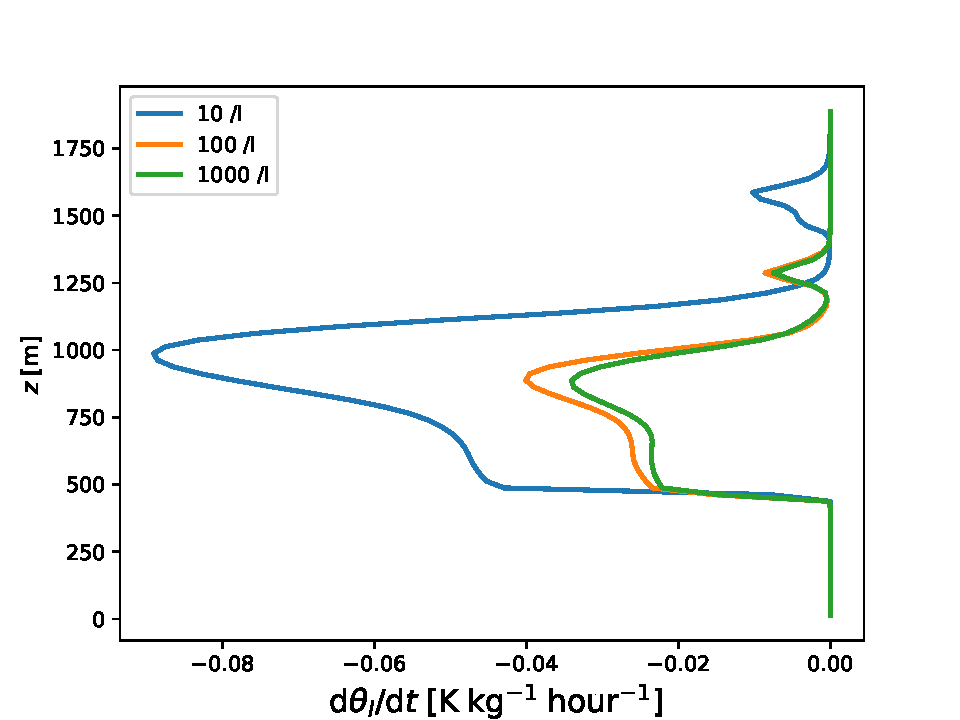
\includegraphics[width=0.52\textwidth]{./figures/prof_tend.pdf}
        \caption[Diagrams and plots]{Here we combine a \textbf{Tikz} diagrams and images. Note that there the references withtin the diagram include active hyeprlinks to other part of this document.}    
      \label{fig:figures}    
 \end{figure}
 
\subsection{Picture}
The figure above is missing labels for some of the panels. Also, we would like to move diagram on the left little bit higher and the one right little bit lower. Instead of opening the figures in some graphical editor, we can perform these tasks \LaTeX with the environment \texttt{picture}. We then encapsule both panels in the environment, and define the coordinates where each panel is located. You can see the result in figure \ref{fig:picture}. 
\begin{lstlisting}[language={[latex]tex}, frame=single,basicstyle=\footnotesize\color{darkgray}, 
  keywordstyle=\bf\color{magenta},
  commentstyle=\color{ForestGreen},  % 
  breaklines=true
  ]
 \begin{picture}(220,180)              % define the size of the picture 
 \put(  0,  20){                       % first panel shifted up by 20 (mm, points, etc.)
          % tikz diagram
     \begin{tikzpicture}[node distance=7mm, auto,]
        %nodes
        \node[point] (market) { \nameref{sec:automatic} };
        \node[point, inner sep=5pt,below=0.5cm of market]
        (conference) {Conferences (see \ref{sec:automatic})};
        % We make a dummy figure to make everything look nice.
        \node[above=of market] (dummy) {};
        \node[right=of dummy] (t) {Poster template}
        edge[pil,bend left=45] (market.east) % edges are used to connect two nodes
        edge[pil, bend left=45] (conference.east); % .east since we want
                                                    % consistent style
        \node[left=of dummy] (g) {Feedback}
        edge[pil, <-,bend right=45] (market.west)
        edge[pil,->, bend left=45] node[auto] {Poster Idea \pageref{fig:standalone} } (t);
    \end{tikzpicture}~\hspace{-2ex}
       % insert the diagram as first panel
 }
 \put(160,  0){                        % first panel shifted right by 160 (mm,
     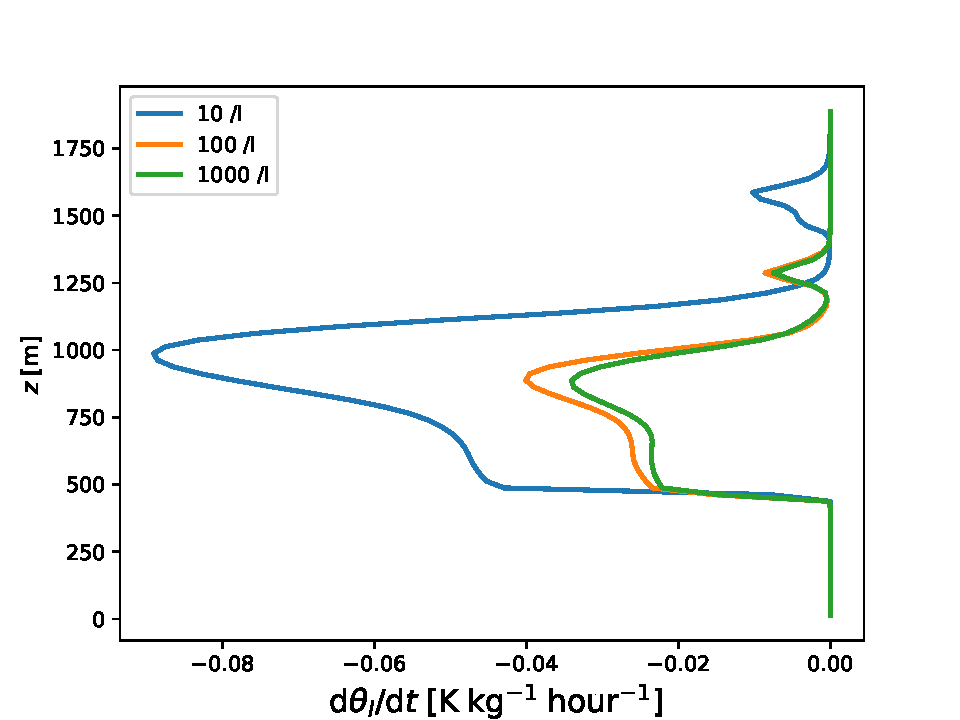
\includegraphics[width=\textwidth]{./figures/prof_tend.pdf} 
 }
 \put(  0,  170){                      % position of the label for the first panel
     {\scriptsize a)}                  % label for the first panel 
 }
 \put(185,  170){                     % position of the label for the second panel
     {\scriptsize b)}                  % label for the second panel 
 }
\end{picture} \caption[Picture package]{Here we take ...
\end{lstlisting}
\begin{figure}[h]
 \begin{picture}(240,175)              % define the size of the picture 
 \put(  0,  20){                       % first panel shifted up by 20 (mm, points, etc.)
          % tikz diagram
     \begin{tikzpicture}[node distance=7mm, auto,]
        %nodes
        \node[point] (market) { \nameref{sec:automatic} };
        \node[point, inner sep=5pt,below=0.5cm of market]
        (conference) {Conferences (see \ref{sec:automatic})};
        % We make a dummy figure to make everything look nice.
        \node[above=of market] (dummy) {};
        \node[right=of dummy] (t) {Poster template}
        edge[pil,bend left=45] (market.east) % edges are used to connect two nodes
        edge[pil, bend left=45] (conference.east); % .east since we want
                                                    % consistent style
        \node[left=of dummy] (g) {Feedback}
        edge[pil, <-,bend right=45] (market.west)
        edge[pil,->, bend left=45] node[auto] {Poster Idea \pageref{fig:standalone} } (t);
    \end{tikzpicture}~\hspace{-2ex}
       % insert the diagram as first panel
 }
 \put(170,  0){                        % first panel shifted right by 160 (mm,
     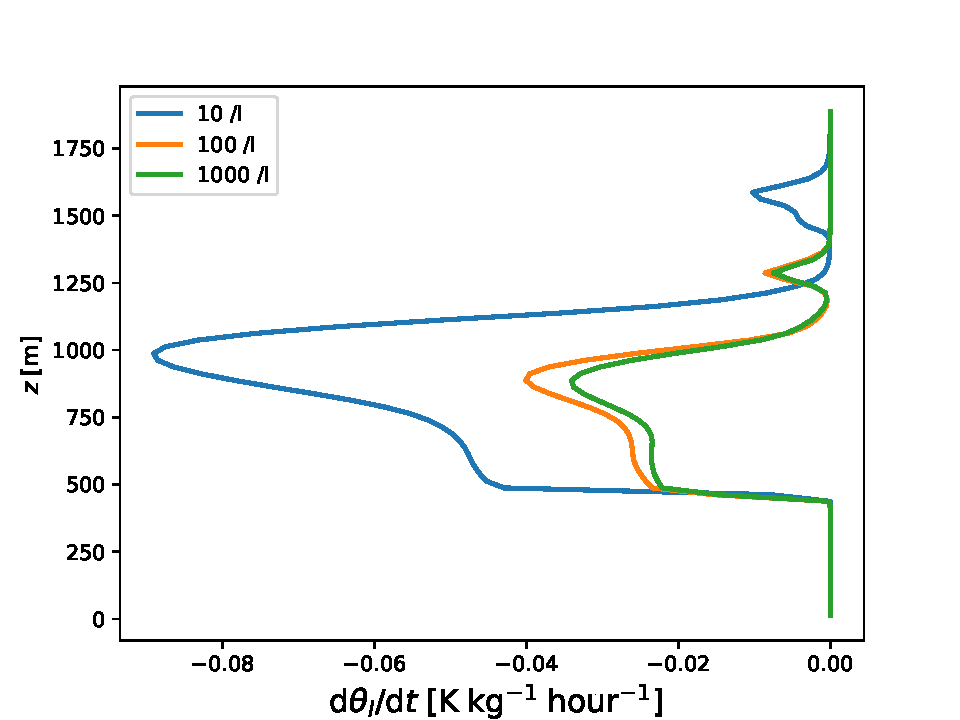
\includegraphics[width=0.52\textwidth]{./figures/prof_tend.pdf}
 }
 \put(  0,  170){                      % position of the label for the first panel
     {\scriptsize a)}                  % label for the first panel 
 }
  \put(185,  170){                     % position of the label for the second panel
     {\scriptsize b)}                  % label for the second panel 
 }
\end{picture}
        \caption[Picture package]{Here we take previous figure and use the picture environment to improve layout and add labels. }    
      \label{fig:picture}   
\end{figure}
 
 \subsection{TikZ}
 
 Figure  \ref{fig:figures} also shows an example of a vector graphics that is defined directly in LaTeX. Out of various available packages, we picked Tikz. In the header of the LaTeX file we should declare which parts of the package we want use:
  
 \begin{lstlisting}[language={[latex]tex}, frame=single,basicstyle=\footnotesize\color{darkgray}, 
  keywordstyle=\bf\color{magenta},
  commentstyle=\color{ForestGreen},  %
  breaklines=true,
  ]
   \usepackage{tikz} 
   \usetikzlibrary{arrows,positioning}
 \end{lstlisting}
 
 Creating the flowchart is relatively simple. From the broad range of graphical function available in the tikz package, we use nodes and edges. In the text fields in the flowchart we can than use various other \LaTeX commands.\\
 We will have a brief look at an example:\\
 
\lstinputlisting[ language={[latex]tex},      % tex syntax, latex option
  caption={Tikz Latex code for Figure \ref{fig:picture}a }, label={code:thislatex}, 
  firstline=2, firstnumber=2, % lastline=387,
  numbers=left, captionpos=b,
  basicstyle=\scriptsize\color{darkgray}, 
  keywordstyle=\bf\color{magenta},
  commentstyle=\color{ForestGreen},  %
  breaklines=true,
  frame=single
]{./latex/diagram.tex}
 
 \subsection{Standalone}
 Some journals request you to upload each figure as a separate pdf. However, what can you do figure consists of multiple panels with labels added in LaTeX? No, you do not need to replot the figure, and you do not need to insert the figure as a separate page. Instead you use \textbf{standalone} class to produce a small image in pdf format. See example \texttt{latex/standalone.tex} of such document.\\
 
 Once you compile a standalone document, you can use it as other graphical elements in pdf format. You can as well include it as an image in this document (see example on the next page).
  
 \begin{figure}[!h] 
     %     % tikz diagram
     \begin{tikzpicture}[node distance=7mm, auto,]
        %nodes
        \node[point] (market) { \nameref{sec:automatic} };
        \node[point, inner sep=5pt,below=0.5cm of market]
        (conference) {Conferences (see \ref{sec:automatic})};
        % We make a dummy figure to make everything look nice.
        \node[above=of market] (dummy) {};
        \node[right=of dummy] (t) {Poster template}
        edge[pil,bend left=45] (market.east) % edges are used to connect two nodes
        edge[pil, bend left=45] (conference.east); % .east since we want
                                                    % consistent style
        \node[left=of dummy] (g) {Feedback}
        edge[pil, <-,bend right=45] (market.west)
        edge[pil,->, bend left=45] node[auto] {Poster Idea \pageref{fig:standalone} } (t);
    \end{tikzpicture}~\hspace{-2ex}

    % ---- directly consrtruction diagram--------------
      % \begin{center}
      \tikzstyle{decision} = [diamond, draw, fill=blue!20, text width=8em, text badly centered, node distance=10em, inner sep=0pt]
      \tikzstyle{block} = [rectangle, draw, fill=blue!20, text width=8em, text centered, rounded corners,node distance=10em ,  minimum height=3em]
      \tikzstyle{block_done} = [rectangle, draw, fill=GreenDone, text width=8em, text centered, node distance=10em, rounded corners, minimum height=3em]
      \tikzstyle{block_special} = [rectangle, draw, fill=lightyellow, text width=8em, text centered, node distance=10em, rounded corners, minimum height=3em]
      \tikzstyle{line} = [draw, -latex']
      \tikzstyle{cloud} = [draw, ellipse, fill=lightyellow, node distance=8em, minimum height=0ex]

      % Tikz Thesis structure diagram
%
  \begin{tikzpicture}[node distance = 4mm, auto] 
    \node [block] (intro)  {1. Introduction};
    \node [block] (theory) at +(8,-0.5) {2. Theory of LEM};
    \node [block_special] (methods) at +(8,-2.5) {3. General Methodology};
    \node [block_special] (idealised) at +(6.5,-4.5) {4. Idealised CAO};
    \node [block_special] (adjusted) at +(6.5,-6.5) {5. Idealised~CAO Adjusted Scenarios};
    \node [block_special] (case_studies) at +(11.5,-7) {6. Case Studies of Cold-Air Outbreaks};  
    \node [block_done] (conclusions) at +(0,-8.5) {7. Conclusions};
    \draw[->,line width=0.8pt] (intro) -- (methods);
    \draw[->,line width=0.8pt] (theory) -- (methods);
    \draw[->,line width=0.8pt] (methods) -- (idealised);
 
    \draw[->,line width=0.8pt] (methods) -- (case_studies);
    \draw[->,line width=0.8pt] (idealised) -- (adjusted);
    \draw[->,line width=0.8pt] (idealised) -- (conclusions);
    \draw[->,line width=0.8pt, dashed](intro) -- (conclusions);
    \draw[-,line width=0.8pt ] (adjusted) -- (6.5, -7.5);
    \draw[-,line width=0.8pt ] (case_studies) -- (11.5, -8.5);
    \draw[->,line width=0.8pt ] (6.5, -7.5) -- (conclusions);
    \draw[->,line width=0.8pt ] (11.5, -8.5) -- (conclusions);
   \end{tikzpicture}~\hspace{-2ex}

   \caption{Here we have a Tikz diagram}
   \label{fig:directly} 
   \end{figure} 
    
    % ---- inserting it from standalone pdf ------------------
   \begin{figure}[!ht]
    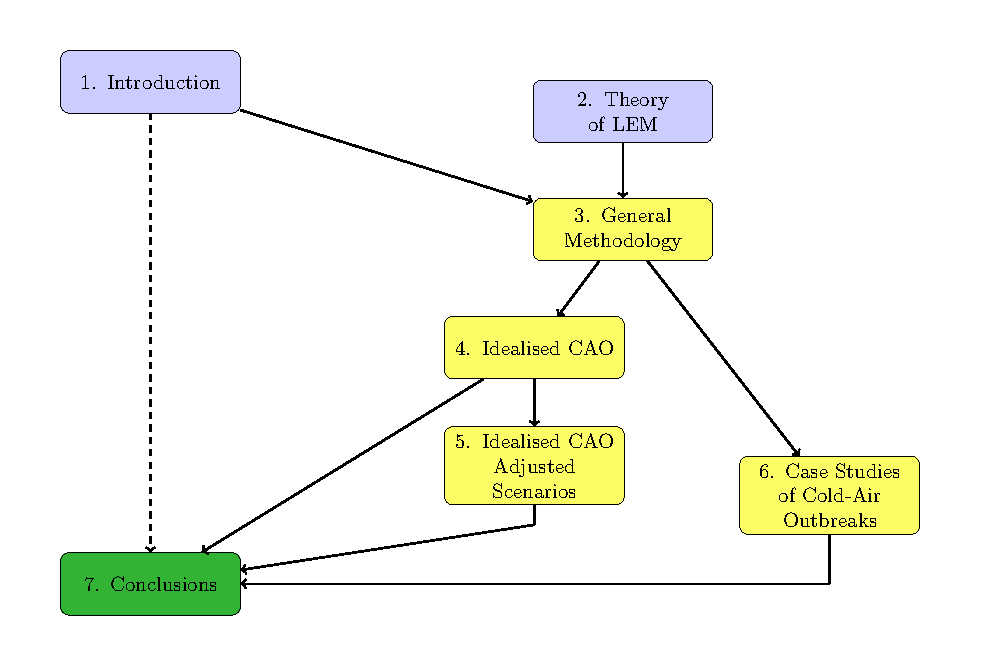
\includegraphics[width=\textwidth]{./latex/standalone.pdf}
        \caption[Diagrams and plots]{We can also compile the figure as separate \textbf{standalone} \index{standalone} pdf and then include it as a graphical element. }  
      \label{fig:standalone}
 \end{figure}

 \newpage 
 
 \section{Customizing Links, References, and Citations}
 So far all the references to the figures, sections, pages, and other counters were marked by brick-red colour of the text. Could we change this style? Not only we can modify the text style of link, the styles can even vary, such as modifying the style of links to other parts of the same document (\nameref{sec:automatic}) and links to \href{https://geomet.uni-koeln.de/en/}{external websites}, as well as links to file such as this document \href{./day1latex.pdf}{./day1latex.pdf}.\\
 
 As you can see in the previous paragraph, we can set different formatting to different types of links. In order to achieve that, we need to include in the header first the package \texttt{hyperref} and then set up options using the command
 \texttt{\textbackslash hypersetup} in the header of the \LaTeX document:\\
 
 \lstinputlisting[ language={[latex]tex},      % tex syntax, latex option
  caption={hypersetup inside in1header.tex}, label={code:hyper}, 
  firstline=97, firstnumber=97, lastline=114, numbers=left, captionpos=b,
  frame=single,
  basicstyle=\scriptsize\color{darkgray}, 
  keywordstyle=\bf\color{magenta},
  commentstyle=\color{ForestGreen},  % 
  breaklines=true
]{./latex/in1header.tex} 
 
 Apart from the basic colour for the links (\texttt{linkcolor}), there are different colours for citation (\texttt{citecolor}), links to files (\texttt{filecolor}), and the web links (\texttt{urlcolor}).
 \pagebreak
 
 \section{Version Control and Comparison}
 We also look at the external tools such as \texttt{latexdiff} that compares \LaTeX files and  \texttt{pdfdiff} that compares \( \ldots \) you know what.\\
 
 Latexdiff can be run as shell command. The arguments are two \LaTeX files, and the output is \LaTeX code which clearly marks which lines of the document differ between the files and which ones are the same. We can redirect the output to a new file.
 
 \begin{lstlisting}[language={bash}, frame=single,basicstyle=\footnotesize
    ,basicstyle=\footnotesize\color{cyan}    % setting font
   ,keywordstyle=\color{magenta}            % setting font for keywords 
   ,stringstyle=\color{brown}
   ,commentstyle=\color{ForestGreen} 
 ]
  latexdiff day1latex.tex day1latex_adjusted1.tex > differences_day1latex.tex
\end{lstlisting}~\vspace{1ex}
%\stepcounter{samplecode}
  


% #4 generating index 
%   \clearpage
%   \phantomsection 
%   \addcontentsline{toc}{section}{Index}  
%   \label{index}  
%   Longer documents sometimes include index pages.
%   \printindex  

\section{Outlook for Wednesday}\label{sec:wednesday}

\begin{itemize}
 \item Tables
 \item Macros
 \item Index
 \item More on version Control
\end{itemize}


 
\label{LastPage}
\newpage


\end{document}
